% Created by tikzDevice version 0.12.3.1 on 2021-12-15 17:50:54
% !TEX encoding = UTF-8 Unicode
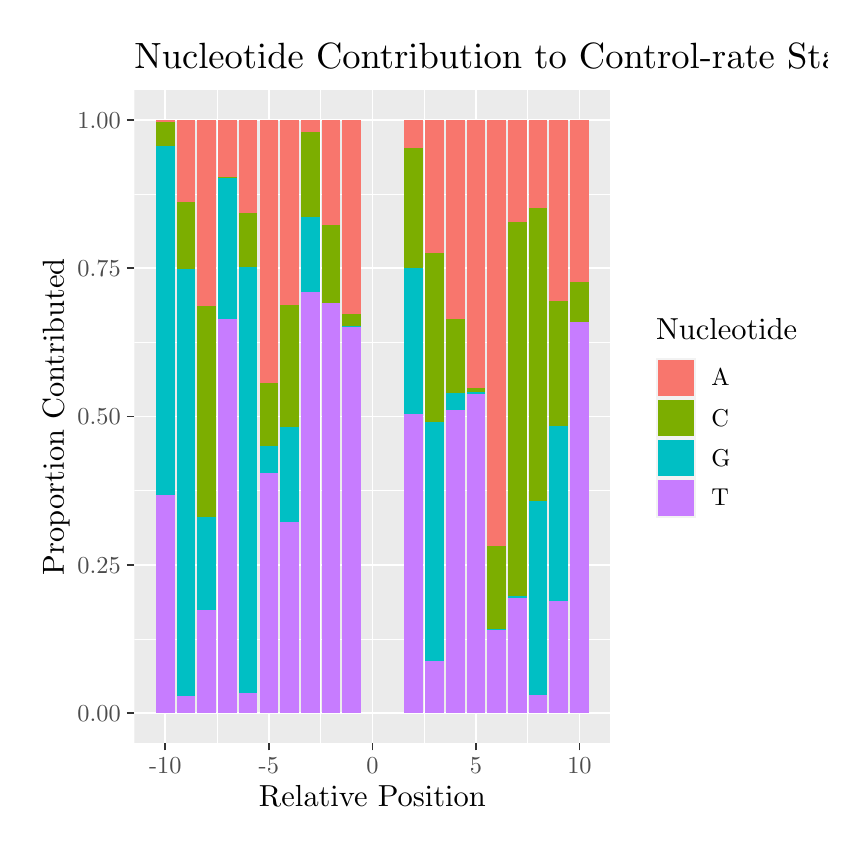
\begin{tikzpicture}[x=1pt,y=1pt]
\definecolor{fillColor}{RGB}{255,255,255}
\path[use as bounding box,fill=fillColor,fill opacity=0.00] (0,0) rectangle (289.08,289.08);
\begin{scope}
\path[clip] (  0.00,  0.00) rectangle (289.08,289.08);
\definecolor{drawColor}{RGB}{255,255,255}
\definecolor{fillColor}{RGB}{255,255,255}

\path[draw=drawColor,line width= 0.6pt,line join=round,line cap=round,fill=fillColor] (  0.00,  0.00) rectangle (289.08,289.08);
\end{scope}
\begin{scope}
\path[clip] ( 38.56, 30.69) rectangle (210.56,266.42);
\definecolor{fillColor}{gray}{0.92}

\path[fill=fillColor] ( 38.56, 30.69) rectangle (210.56,266.42);
\definecolor{drawColor}{RGB}{255,255,255}

\path[draw=drawColor,line width= 0.3pt,line join=round] ( 38.56, 68.19) --
	(210.56, 68.19);

\path[draw=drawColor,line width= 0.3pt,line join=round] ( 38.56,121.77) --
	(210.56,121.77);

\path[draw=drawColor,line width= 0.3pt,line join=round] ( 38.56,175.34) --
	(210.56,175.34);

\path[draw=drawColor,line width= 0.3pt,line join=round] ( 38.56,228.92) --
	(210.56,228.92);

\path[draw=drawColor,line width= 0.3pt,line join=round] ( 68.45, 30.69) --
	( 68.45,266.42);

\path[draw=drawColor,line width= 0.3pt,line join=round] (105.85, 30.69) --
	(105.85,266.42);

\path[draw=drawColor,line width= 0.3pt,line join=round] (143.26, 30.69) --
	(143.26,266.42);

\path[draw=drawColor,line width= 0.3pt,line join=round] (180.67, 30.69) --
	(180.67,266.42);

\path[draw=drawColor,line width= 0.6pt,line join=round] ( 38.56, 41.40) --
	(210.56, 41.40);

\path[draw=drawColor,line width= 0.6pt,line join=round] ( 38.56, 94.98) --
	(210.56, 94.98);

\path[draw=drawColor,line width= 0.6pt,line join=round] ( 38.56,148.55) --
	(210.56,148.55);

\path[draw=drawColor,line width= 0.6pt,line join=round] ( 38.56,202.13) --
	(210.56,202.13);

\path[draw=drawColor,line width= 0.6pt,line join=round] ( 38.56,255.71) --
	(210.56,255.71);

\path[draw=drawColor,line width= 0.6pt,line join=round] ( 49.74, 30.69) --
	( 49.74,266.42);

\path[draw=drawColor,line width= 0.6pt,line join=round] ( 87.15, 30.69) --
	( 87.15,266.42);

\path[draw=drawColor,line width= 0.6pt,line join=round] (124.56, 30.69) --
	(124.56,266.42);

\path[draw=drawColor,line width= 0.6pt,line join=round] (161.97, 30.69) --
	(161.97,266.42);

\path[draw=drawColor,line width= 0.6pt,line join=round] (199.38, 30.69) --
	(199.38,266.42);
\definecolor{fillColor}{RGB}{248,118,109}

\path[fill=fillColor] ( 46.37,254.86) rectangle ( 53.11,255.71);
\definecolor{fillColor}{RGB}{124,174,0}

\path[fill=fillColor] ( 46.37,246.39) rectangle ( 53.11,254.86);
\definecolor{fillColor}{RGB}{0,191,196}

\path[fill=fillColor] ( 46.37,120.37) rectangle ( 53.11,246.39);
\definecolor{fillColor}{RGB}{199,124,255}

\path[fill=fillColor] ( 46.37, 41.40) rectangle ( 53.11,120.37);
\definecolor{fillColor}{RGB}{248,118,109}

\path[fill=fillColor] ( 53.86,226.11) rectangle ( 60.59,255.71);
\definecolor{fillColor}{RGB}{124,174,0}

\path[fill=fillColor] ( 53.86,201.80) rectangle ( 60.59,226.11);
\definecolor{fillColor}{RGB}{0,191,196}

\path[fill=fillColor] ( 53.86, 47.75) rectangle ( 60.59,201.80);
\definecolor{fillColor}{RGB}{199,124,255}

\path[fill=fillColor] ( 53.86, 41.40) rectangle ( 60.59, 47.75);
\definecolor{fillColor}{RGB}{248,118,109}

\path[fill=fillColor] ( 61.34,188.39) rectangle ( 68.07,255.71);
\definecolor{fillColor}{RGB}{124,174,0}

\path[fill=fillColor] ( 61.34,112.29) rectangle ( 68.07,188.39);
\definecolor{fillColor}{RGB}{0,191,196}

\path[fill=fillColor] ( 61.34, 78.48) rectangle ( 68.07,112.29);
\definecolor{fillColor}{RGB}{199,124,255}

\path[fill=fillColor] ( 61.34, 41.40) rectangle ( 68.07, 78.48);
\definecolor{fillColor}{RGB}{248,118,109}

\path[fill=fillColor] ( 68.82,235.11) rectangle ( 75.55,255.71);
\definecolor{fillColor}{RGB}{124,174,0}

\path[fill=fillColor] ( 68.82,234.70) rectangle ( 75.55,235.11);
\definecolor{fillColor}{RGB}{199,124,255}

\path[fill=fillColor] ( 68.82, 41.40) rectangle ( 75.55,183.65);
\definecolor{fillColor}{RGB}{0,191,196}

\path[fill=fillColor] ( 68.82,183.65) rectangle ( 75.55,234.70);
\definecolor{fillColor}{RGB}{248,118,109}

\path[fill=fillColor] ( 76.30,221.95) rectangle ( 83.04,255.71);
\definecolor{fillColor}{RGB}{124,174,0}

\path[fill=fillColor] ( 76.30,202.68) rectangle ( 83.04,221.95);
\definecolor{fillColor}{RGB}{199,124,255}

\path[fill=fillColor] ( 76.30, 41.40) rectangle ( 83.04, 48.55);
\definecolor{fillColor}{RGB}{0,191,196}

\path[fill=fillColor] ( 76.30, 48.55) rectangle ( 83.04,202.68);
\definecolor{fillColor}{RGB}{248,118,109}

\path[fill=fillColor] ( 83.78,160.53) rectangle ( 90.52,255.71);
\definecolor{fillColor}{RGB}{124,174,0}

\path[fill=fillColor] ( 83.78,137.79) rectangle ( 90.52,160.53);
\definecolor{fillColor}{RGB}{0,191,196}

\path[fill=fillColor] ( 83.78,128.09) rectangle ( 90.52,137.79);
\definecolor{fillColor}{RGB}{199,124,255}

\path[fill=fillColor] ( 83.78, 41.40) rectangle ( 90.52,128.09);
\definecolor{fillColor}{RGB}{248,118,109}

\path[fill=fillColor] ( 91.27,188.99) rectangle ( 98.00,255.71);
\definecolor{fillColor}{RGB}{124,174,0}

\path[fill=fillColor] ( 91.27,144.72) rectangle ( 98.00,188.99);
\definecolor{fillColor}{RGB}{0,191,196}

\path[fill=fillColor] ( 91.27,110.43) rectangle ( 98.00,144.72);
\definecolor{fillColor}{RGB}{199,124,255}

\path[fill=fillColor] ( 91.27, 41.40) rectangle ( 98.00,110.43);
\definecolor{fillColor}{RGB}{248,118,109}

\path[fill=fillColor] ( 98.75,251.53) rectangle (105.48,255.71);
\definecolor{fillColor}{RGB}{124,174,0}

\path[fill=fillColor] ( 98.75,220.82) rectangle (105.48,251.53);
\definecolor{fillColor}{RGB}{0,191,196}

\path[fill=fillColor] ( 98.75,193.42) rectangle (105.48,220.82);
\definecolor{fillColor}{RGB}{199,124,255}

\path[fill=fillColor] ( 98.75, 41.40) rectangle (105.48,193.42);
\definecolor{fillColor}{RGB}{248,118,109}

\path[fill=fillColor] (106.23,217.77) rectangle (112.96,255.71);
\definecolor{fillColor}{RGB}{124,174,0}

\path[fill=fillColor] (106.23,189.66) rectangle (112.96,217.77);
\definecolor{fillColor}{RGB}{0,191,196}

\path[fill=fillColor] (106.23,189.61) rectangle (112.96,189.66);
\definecolor{fillColor}{RGB}{199,124,255}

\path[fill=fillColor] (106.23, 41.40) rectangle (112.96,189.61);
\definecolor{fillColor}{RGB}{248,118,109}

\path[fill=fillColor] (113.71,185.55) rectangle (120.44,255.71);
\definecolor{fillColor}{RGB}{124,174,0}

\path[fill=fillColor] (113.71,181.11) rectangle (120.44,185.55);
\definecolor{fillColor}{RGB}{0,191,196}

\path[fill=fillColor] (113.71,180.78) rectangle (120.44,181.11);
\definecolor{fillColor}{RGB}{199,124,255}

\path[fill=fillColor] (113.71, 41.40) rectangle (120.44,180.78);
\definecolor{fillColor}{RGB}{248,118,109}

\path[fill=fillColor] (136.16,245.71) rectangle (142.89,255.71);
\definecolor{fillColor}{RGB}{124,174,0}

\path[fill=fillColor] (136.16,202.41) rectangle (142.89,245.71);
\definecolor{fillColor}{RGB}{0,191,196}

\path[fill=fillColor] (136.16,149.56) rectangle (142.89,202.41);
\definecolor{fillColor}{RGB}{199,124,255}

\path[fill=fillColor] (136.16, 41.40) rectangle (142.89,149.56);
\definecolor{fillColor}{RGB}{248,118,109}

\path[fill=fillColor] (143.64,207.60) rectangle (150.37,255.71);
\definecolor{fillColor}{RGB}{124,174,0}

\path[fill=fillColor] (143.64,146.53) rectangle (150.37,207.60);
\definecolor{fillColor}{RGB}{199,124,255}

\path[fill=fillColor] (143.64, 41.40) rectangle (150.37, 60.31);
\definecolor{fillColor}{RGB}{0,191,196}

\path[fill=fillColor] (143.64, 60.31) rectangle (150.37,146.53);
\definecolor{fillColor}{RGB}{248,118,109}

\path[fill=fillColor] (151.12,183.93) rectangle (157.85,255.71);
\definecolor{fillColor}{RGB}{124,174,0}

\path[fill=fillColor] (151.12,156.96) rectangle (157.85,183.93);
\definecolor{fillColor}{RGB}{0,191,196}

\path[fill=fillColor] (151.12,151.02) rectangle (157.85,156.96);
\definecolor{fillColor}{RGB}{199,124,255}

\path[fill=fillColor] (151.12, 41.40) rectangle (157.85,151.02);
\definecolor{fillColor}{RGB}{248,118,109}

\path[fill=fillColor] (158.60,158.89) rectangle (165.34,255.71);
\definecolor{fillColor}{RGB}{124,174,0}

\path[fill=fillColor] (158.60,157.50) rectangle (165.34,158.89);
\definecolor{fillColor}{RGB}{0,191,196}

\path[fill=fillColor] (158.60,156.75) rectangle (165.34,157.50);
\definecolor{fillColor}{RGB}{199,124,255}

\path[fill=fillColor] (158.60, 41.40) rectangle (165.34,156.75);
\definecolor{fillColor}{RGB}{248,118,109}

\path[fill=fillColor] (166.08,101.74) rectangle (172.82,255.71);
\definecolor{fillColor}{RGB}{124,174,0}

\path[fill=fillColor] (166.08, 71.91) rectangle (172.82,101.74);
\definecolor{fillColor}{RGB}{199,124,255}

\path[fill=fillColor] (166.08, 41.40) rectangle (172.82, 71.73);
\definecolor{fillColor}{RGB}{0,191,196}

\path[fill=fillColor] (166.08, 71.73) rectangle (172.82, 71.91);
\definecolor{fillColor}{RGB}{248,118,109}

\path[fill=fillColor] (173.57,219.01) rectangle (180.30,255.71);
\definecolor{fillColor}{RGB}{124,174,0}

\path[fill=fillColor] (173.57, 83.57) rectangle (180.30,219.01);
\definecolor{fillColor}{RGB}{199,124,255}

\path[fill=fillColor] (173.57, 41.40) rectangle (180.30, 83.14);
\definecolor{fillColor}{RGB}{0,191,196}

\path[fill=fillColor] (173.57, 83.14) rectangle (180.30, 83.57);
\definecolor{fillColor}{RGB}{248,118,109}

\path[fill=fillColor] (181.05,223.75) rectangle (187.78,255.71);
\definecolor{fillColor}{RGB}{124,174,0}

\path[fill=fillColor] (181.05,118.12) rectangle (187.78,223.75);
\definecolor{fillColor}{RGB}{0,191,196}

\path[fill=fillColor] (181.05, 48.01) rectangle (187.78,118.12);
\definecolor{fillColor}{RGB}{199,124,255}

\path[fill=fillColor] (181.05, 41.40) rectangle (187.78, 48.01);
\definecolor{fillColor}{RGB}{248,118,109}

\path[fill=fillColor] (188.53,190.26) rectangle (195.26,255.71);
\definecolor{fillColor}{RGB}{124,174,0}

\path[fill=fillColor] (188.53,144.97) rectangle (195.26,190.26);
\definecolor{fillColor}{RGB}{0,191,196}

\path[fill=fillColor] (188.53, 81.79) rectangle (195.26,144.97);
\definecolor{fillColor}{RGB}{199,124,255}

\path[fill=fillColor] (188.53, 41.40) rectangle (195.26, 81.79);
\definecolor{fillColor}{RGB}{248,118,109}

\path[fill=fillColor] (196.01,197.04) rectangle (202.75,255.71);
\definecolor{fillColor}{RGB}{124,174,0}

\path[fill=fillColor] (196.01,182.83) rectangle (202.75,197.04);
\definecolor{fillColor}{RGB}{0,191,196}

\path[fill=fillColor] (196.01,182.83) rectangle (202.75,182.83);
\definecolor{fillColor}{RGB}{199,124,255}

\path[fill=fillColor] (196.01, 41.40) rectangle (202.75,182.83);
\end{scope}
\begin{scope}
\path[clip] (  0.00,  0.00) rectangle (289.08,289.08);
\definecolor{drawColor}{gray}{0.30}

\node[text=drawColor,anchor=base east,inner sep=0pt, outer sep=0pt, scale=  0.88] at ( 33.61, 38.37) {0.00};

\node[text=drawColor,anchor=base east,inner sep=0pt, outer sep=0pt, scale=  0.88] at ( 33.61, 91.95) {0.25};

\node[text=drawColor,anchor=base east,inner sep=0pt, outer sep=0pt, scale=  0.88] at ( 33.61,145.52) {0.50};

\node[text=drawColor,anchor=base east,inner sep=0pt, outer sep=0pt, scale=  0.88] at ( 33.61,199.10) {0.75};

\node[text=drawColor,anchor=base east,inner sep=0pt, outer sep=0pt, scale=  0.88] at ( 33.61,252.68) {1.00};
\end{scope}
\begin{scope}
\path[clip] (  0.00,  0.00) rectangle (289.08,289.08);
\definecolor{drawColor}{gray}{0.20}

\path[draw=drawColor,line width= 0.6pt,line join=round] ( 35.81, 41.40) --
	( 38.56, 41.40);

\path[draw=drawColor,line width= 0.6pt,line join=round] ( 35.81, 94.98) --
	( 38.56, 94.98);

\path[draw=drawColor,line width= 0.6pt,line join=round] ( 35.81,148.55) --
	( 38.56,148.55);

\path[draw=drawColor,line width= 0.6pt,line join=round] ( 35.81,202.13) --
	( 38.56,202.13);

\path[draw=drawColor,line width= 0.6pt,line join=round] ( 35.81,255.71) --
	( 38.56,255.71);
\end{scope}
\begin{scope}
\path[clip] (  0.00,  0.00) rectangle (289.08,289.08);
\definecolor{drawColor}{gray}{0.20}

\path[draw=drawColor,line width= 0.6pt,line join=round] ( 49.74, 27.94) --
	( 49.74, 30.69);

\path[draw=drawColor,line width= 0.6pt,line join=round] ( 87.15, 27.94) --
	( 87.15, 30.69);

\path[draw=drawColor,line width= 0.6pt,line join=round] (124.56, 27.94) --
	(124.56, 30.69);

\path[draw=drawColor,line width= 0.6pt,line join=round] (161.97, 27.94) --
	(161.97, 30.69);

\path[draw=drawColor,line width= 0.6pt,line join=round] (199.38, 27.94) --
	(199.38, 30.69);
\end{scope}
\begin{scope}
\path[clip] (  0.00,  0.00) rectangle (289.08,289.08);
\definecolor{drawColor}{gray}{0.30}

\node[text=drawColor,anchor=base,inner sep=0pt, outer sep=0pt, scale=  0.88] at ( 49.74, 19.68) {-10};

\node[text=drawColor,anchor=base,inner sep=0pt, outer sep=0pt, scale=  0.88] at ( 87.15, 19.68) {-5};

\node[text=drawColor,anchor=base,inner sep=0pt, outer sep=0pt, scale=  0.88] at (124.56, 19.68) {0};

\node[text=drawColor,anchor=base,inner sep=0pt, outer sep=0pt, scale=  0.88] at (161.97, 19.68) {5};

\node[text=drawColor,anchor=base,inner sep=0pt, outer sep=0pt, scale=  0.88] at (199.38, 19.68) {10};
\end{scope}
\begin{scope}
\path[clip] (  0.00,  0.00) rectangle (289.08,289.08);
\definecolor{drawColor}{RGB}{0,0,0}

\node[text=drawColor,anchor=base,inner sep=0pt, outer sep=0pt, scale=  1.10] at (124.56,  7.64) {Relative Position};
\end{scope}
\begin{scope}
\path[clip] (  0.00,  0.00) rectangle (289.08,289.08);
\definecolor{drawColor}{RGB}{0,0,0}

\node[text=drawColor,rotate= 90.00,anchor=base,inner sep=0pt, outer sep=0pt, scale=  1.10] at ( 13.08,148.55) {Proportion Contributed};
\end{scope}
\begin{scope}
\path[clip] (  0.00,  0.00) rectangle (289.08,289.08);
\definecolor{fillColor}{RGB}{255,255,255}

\path[fill=fillColor] (221.56,106.54) rectangle (283.58,190.57);
\end{scope}
\begin{scope}
\path[clip] (  0.00,  0.00) rectangle (289.08,289.08);
\definecolor{drawColor}{RGB}{0,0,0}

\node[text=drawColor,anchor=base west,inner sep=0pt, outer sep=0pt, scale=  1.10] at (227.06,176.42) {Nucleotide};
\end{scope}
\begin{scope}
\path[clip] (  0.00,  0.00) rectangle (289.08,289.08);
\definecolor{fillColor}{gray}{0.95}

\path[fill=fillColor] (227.06,155.40) rectangle (241.52,169.86);
\end{scope}
\begin{scope}
\path[clip] (  0.00,  0.00) rectangle (289.08,289.08);
\definecolor{fillColor}{RGB}{248,118,109}

\path[fill=fillColor] (227.78,156.11) rectangle (240.81,169.14);
\end{scope}
\begin{scope}
\path[clip] (  0.00,  0.00) rectangle (289.08,289.08);
\definecolor{fillColor}{gray}{0.95}

\path[fill=fillColor] (227.06,140.95) rectangle (241.52,155.40);
\end{scope}
\begin{scope}
\path[clip] (  0.00,  0.00) rectangle (289.08,289.08);
\definecolor{fillColor}{RGB}{124,174,0}

\path[fill=fillColor] (227.78,141.66) rectangle (240.81,154.69);
\end{scope}
\begin{scope}
\path[clip] (  0.00,  0.00) rectangle (289.08,289.08);
\definecolor{fillColor}{gray}{0.95}

\path[fill=fillColor] (227.06,126.49) rectangle (241.52,140.95);
\end{scope}
\begin{scope}
\path[clip] (  0.00,  0.00) rectangle (289.08,289.08);
\definecolor{fillColor}{RGB}{0,191,196}

\path[fill=fillColor] (227.78,127.20) rectangle (240.81,140.24);
\end{scope}
\begin{scope}
\path[clip] (  0.00,  0.00) rectangle (289.08,289.08);
\definecolor{fillColor}{gray}{0.95}

\path[fill=fillColor] (227.06,112.04) rectangle (241.52,126.49);
\end{scope}
\begin{scope}
\path[clip] (  0.00,  0.00) rectangle (289.08,289.08);
\definecolor{fillColor}{RGB}{199,124,255}

\path[fill=fillColor] (227.78,112.75) rectangle (240.81,125.78);
\end{scope}
\begin{scope}
\path[clip] (  0.00,  0.00) rectangle (289.08,289.08);
\definecolor{drawColor}{RGB}{0,0,0}

\node[text=drawColor,anchor=base west,inner sep=0pt, outer sep=0pt, scale=  0.88] at (247.02,159.60) {A};
\end{scope}
\begin{scope}
\path[clip] (  0.00,  0.00) rectangle (289.08,289.08);
\definecolor{drawColor}{RGB}{0,0,0}

\node[text=drawColor,anchor=base west,inner sep=0pt, outer sep=0pt, scale=  0.88] at (247.02,145.14) {C};
\end{scope}
\begin{scope}
\path[clip] (  0.00,  0.00) rectangle (289.08,289.08);
\definecolor{drawColor}{RGB}{0,0,0}

\node[text=drawColor,anchor=base west,inner sep=0pt, outer sep=0pt, scale=  0.88] at (247.02,130.69) {G};
\end{scope}
\begin{scope}
\path[clip] (  0.00,  0.00) rectangle (289.08,289.08);
\definecolor{drawColor}{RGB}{0,0,0}

\node[text=drawColor,anchor=base west,inner sep=0pt, outer sep=0pt, scale=  0.88] at (247.02,116.24) {T};
\end{scope}
\begin{scope}
\path[clip] (  0.00,  0.00) rectangle (289.08,289.08);
\definecolor{drawColor}{RGB}{0,0,0}

\node[text=drawColor,anchor=base west,inner sep=0pt, outer sep=0pt, scale=  1.32] at ( 38.56,274.49) {Nucleotide Contribution to Control-rate Statistic: cpg-GC-AT};
\end{scope}
\end{tikzpicture}
